\documentclass[12pt]{article}

\usepackage{times,graphicx,rotating}
%times,palatino,bookman, palatino, newcent

\usepackage{geometry}
 \geometry{ a4paper, total={210mm,297mm},
 left=25mm,
 right=25mm,
 top=20mm,
 bottom=20mm,
 }


\begin{document}

\title{FER\reflectbox{R}E User's Guide}

\date{\today}
\author{C. Allende Prieto}

\maketitle

FERRE is a data analysis code written in FORTRAN90. 
It matches models to data, taking a set of observations 
and identifying the model parameters that best
reproduce the data, in a chi-squared sense. 
Model predictions are to be given as an array whose values are a function of 
the model parameters, i.e. numerically. 
FERRE holds this array in memory, or in a direct-access binary file,
and interpolates in it. The code returns, in addition to the optimal 
set of parameters, their error covariance, and the corresponding model prediction. 

\tableofcontents

\newpage

\section{Introduction}
\label{intro}

Using models to interpret observations is a very common task in 
science. Models may be sophisticated, sometimes the result 
of solving complex sets equations, and can only be evaluated numerically 
in some cases. The data sets to be analyzed may be large, regarding both 
the number of objects and the data per object. And so can be the models, 
which may involve a large number of parameters. 

FERRE matches physical models to observed data. It was created to 
deal with the common problem of having numerical models that are
costly to evaluate, and need to be used to interpret large data sets.
FERRE provides flexibility to search for all model parameters, or 
only some them holding constant the others. The code is written
to be truly N-dimensional and fast. The merit function to evaluate 
agreement between models ${m_i}$ and observations ${o_i}$ 
(with uncertainties ${\sigma_i(o)}$) is the $\chi^2$ square
\begin{equation}
\chi^2 = \sum_i \frac{1}{\sigma_i^2(o)} (m_i - o_i)^2.
\end{equation}

Models are to be
encapsulated in a multi-dimensional array, with as many dimensions
as parameters. The model array is held in memory for speed, but it can
also be written in disk ans used as a data base. Models are interpolated with a choice
of algorithms (linear, Bezier quadratic, cubic, and cubic splines), with 
interpolations carried out in a sequential fashion. 

Several optimization algorithms are available to search for the 
best-fitting model parameters: 
the Nelder-Mead algorithm (Nelder \& Mead 1965), 
the  Boender-Timmer-Rinnoy Kan global algorithm (Boender et al. 1982), 
Powell's UOBYQA algorithm (Powell 2000), 
a Truncated Newton algorithm (Dembo \& Steihaug 1983), 
or a weighted sum over the parameters space. Several schemes are also available 
for estimating error bars on the derived abundances. 

Some applications can benefit from data compression applied to models based on 
Principal Component Analysis, and parallelization
over multiple cores, which are both handled in a way that is
fairly transparent to users.
FERRE has a history of successful applications to the analysis of
astronomical spectra since 2003 (see \S \ref{literature}).

\section{Optaining and compiling the code}
\label{compiling}

FERRE is free software. It is written in FORTRAN90, and parallelized
with OpenMP. It is been successfully compiled with gfortran, g95, 
the Intel compiler (ifort), the  Sun Studio Compiler, the PGI compiler, 
the IBM compiler (xlf90), and a few other.

The code can be obtained from \\
{\tt http://hebe.as.utexas.edu/ferre} \\
Once the tar ball with the source code is downloaded and unpacked, 
you should end up with three
folders: src (the 'code'), test (test data), 
and doc (this manual). Change directories to src and invoke
make to compile the code  \\
$>$cd  ferre/src \\
$>$make  \\
\noindent and you should end up with two executables, 
one for FERRE ('a.out') and one for  converting
model grids from ASCII format to (direct-access) binaries.

\section{Running the code}
\label{running}

To run FERRE we need a model grid (see Section \ref{grid}), a control
file ({\tt input.nml}; see \S \ref{nml}), 
and input data files (see \S \ref{input}).
Once all these are in place, we simply need to invoke the ferre executable
from a working directory, where the aforementioned files 
(or symbolic links to them) need to be. After describing the format 
for the input files, we illustrate how to run FERRE with examples
in Section \ref{test}.

\section{Model grid}
\label{grid}

In order to run FERRE you need to make your model predictions available 
as a data file. 
The model of your choice will predict
the same quantities that we have observations
for, as a function of the model parameters. This is precisely what
is in the file that contains the model grid, 
a multi-dimensional array
with as many dimensions as model parameters. In general, there will 
be multiple observations, e.g. multiple quantities or the same quantity
observed as a function of time. This gives one additional dimension
to the model grid. The grid must be perfectly regular, 
i.e. if two parameters are considered, and the first one is sampled
with 4 values  and  the second one with 6 values, the grid will 
have 24 models, corresponding to all possible combinations of
the values for the two parameters.    

The format of the file that contains the model grid (a.k.a. the SYNTH
module) is very simple. Each model prediction, corresponding to a given
combination of parameters, takes a full line in the file. In our previous
example with two parameters, and 4 and 6 values for each of the parameters,
respectively, the file would have 24 lines. If the array of observed
quantities has 20 elements, then each line in the file will have 20 
columns. The numbers (model predictions) are preceded by
a header explaining the contents.   The order of the model predictions
can be easily recovered. Since the grid is regular, a series of
nested loops, according to the information  specified in the file header, 
gives  the values of the parameters that correspond to each line 
in the file.    

An example may help. If we are dealing with spectroscopy of stars,
and the observations are relative photon fluxes at different wavelengths,
our model grid could include spectra predicted as a function of 
effective temperature, surface gravity, and 
metallicity\footnote{Most stars are approximately made of 80\%  H, 18\% He, 
and about 2\% of the rest of elements. It is the latter group of elements, 
those heavier than He, what matters the most for shaping stellar spectra, 
and as such it is one of the parameters that needs to be considered in 
models.}.
If we consider a model grid of spectra that includes 100 wavelengths, 
with 10 effective temperatures, 10 gravities,
and 10 metallicities, our grid file will have 1000 lines, with 100 columns each.

Since the model grids are perfectly regular, with constant steps in the parameters
that define them, a few quantities can describe them. Those quantities
are provided in the header of the file. For example, the values that
correspond to each of the parameters can be described with a linear
equation, $Y=aX+b$, one for each parameter.  The relevant coefficients  
are given  in the file header, identified with the keywords 
LLIMITS (coefficient $b$) and STEPS (coefficient $a$). 

The model grid file always begins with the line \\
{\tt \&SYNTH}\\
which tells FERRE the header is a name list with that name.
Only a few of the keywords possible in the grid header are mandatory: 
\begin{itemize}
\item n\_of\_dim: Number of dimensions (parameters) of the model grid,
\item n\_p: An array with the number of data points in the grid for each 
dimension (it is an array with as many elements as dimensions the grid has),
\item npix: Number of data points per sample (frequencies for
	spectroscopy),
\item llimits: Array with the minimum values for each of the model parameters, and 
\item steps: Array with the steps (difference between two consecutive nodes) 
for each dimension.
\end{itemize}

These, and other optional keywords
are listed in Table 1. Many of the optional keywords are
intended to deal with spectroscopic data; they are mainly 
for tracking the contents of the file, and they are clearly
marked in Table 1.

\begin{table}
\label{t1}
\caption{Parameters that can be used in the header of a FERRE model grid. 
Only the first few at the top of the list are usually required.}
\begin{tabular}{lcl}
\hline
Parameter  & Type (elements) & Meaning \\
\hline
\hline
Mandatory  & Parameters \\
\hline
n\_of\_dim & integer            & Number of dimensions \\
n\_p        & integer (n\_of\_dim)  & Number of data points per dimensions \\
npix       & integer            & Number of observations per sample \\
llimits    & integer (n\_of\_dim)  & Lower limits for the model parameter arrays \\
steps      & integer (n\_of\_dim)  & Steps for each of the parameter arrays \\
\hline
Optional   & Parameters \\
\hline
multi      &  integer              & Number of headers after the main one \\
synthfile\_internal &  string       & Internal name of the model grid file \\
id         &  string       & File identifier \\
date       &  string       & Date when the file was assembled     \\
npca       &  integer (*)  & Number of PCA components per PCA section \\
label      &  string (n\_of\_dim)  &  Tags identifying the parameters of the model \\
transposed    & integer    & A value $>0$ indicates data are transposed \\
comments1...6     &  Comment fields \\
\hline
Optional   & Parameters  & intended for use with spectroscopic data \\
\hline
wave       & float (2)     & Coeffs. in $\lambda =$ wave(1) + (i-1)*wave(2) (i=1...npix) \\
logw       & integer       & Values of 0/1/2 indicate we use $\lambda$/log10($\lambda$)/ln($\lambda$) \\
vacuum     &  integer      & Values of 0/1 indicate air/vacuum wavelengths \\
resolution    & float      & Resolving power ($\lambda$/FWHM) of the spectra \\
original\_sampling    & float & Velocity sampling in original calculations (km/s) \\
synspec    &  integer      & When $>0$ indicates spectra computed with Synspec \\
modo    & integer          & When synspec=1, this the value of 'imode' \\
invalid\_code    &  float  & Value used to indicate data are unavailable \\
constant    & float  &   Constant value subtracted to the entire grid \\
continuum    & float (4)  & Coefficients used for continuum normalization \\
precontinuum    &  float (4) & Coefficients for a pre-normalization \\
file\_data19    & string & Atomic line list used in the synthesis \\
file\_data20    & string & Molecular line list used in the synthesis \\
\hline
\end{tabular} 
\end{table}

\section{Control file}
\label{nml}

The control file is named {\tt input.nml}. It tells FERRE what to do:
the dimensions of the problem, the name of the input files,
how to search for the solutions, or how to interpolate. The control files
must always begin with the line \\
{\tt \&LISTA}\\
As with the model grid file, only a few of the keywords are mandatory:
\begin{itemize}
\item ndim: Number of dimensions/parameters the problem has 
  (must match n\_of\_dim in the model grid file), 
\item nov: Number of parameters to vary (those we wish to search for; 
  the remainder of the parameters will be held at constant values of the user's choice), 
\item indv: Array of indices corresponding to the parameters to vary 
  (following the order given in the model grid), 
\item synthfile(1): File name for the model grid (can use several), 
\item pfile: Parameter file (name of the file with 'input' parameters; 
  see \S \ref{input} for details), 
\item ffile: Data file (name of the file with the observations; 
  see \S \ref{input} for details), 
\item erfile: Error data file (name of the file with the uncertainties 
  associated to the data file, in the same format; see \S \ref{input} for details), 
\item opfile: Output parameter file (output from FERRE, which contains the
best-fitting model parameters for each sample), and 
\item offile: Output data file (output from FERRE, containing the best-fitting 
  model predictions for each sample).
\end{itemize}

These and the remainder of the 
possible keywords are explained in Table 2.

\begin{table}
\label{t2}
\caption{Parameters that can be used in the FERRE control file ({\tt input.nml}). 
Only the first few at the top of the list are mandatory (default values in parenthesis).}
\begin{tabular}{lcl}
\hline
Parameter  & Type (elements) & Meaning \\
\hline
\hline
Mandatory  & Parameters \\
\hline
ndim     & integer            & Number of dimensions/parameters (should match 
n\_of\_dim) \\
nov      & integer            & Number of parameters to search \\
         &                    & nov=0 if we just want to interpolate in the grid \\
indv     & integer (nov)         & Array with the indices for the parameters to search \\
synthfile & string (*)           & File name(s) for the model grid(s) \\
pfile     &   string             & Name of the input parameter file \\
ffile     &   string             & Name of the input data file (the observations we want to model) \\
erfile    &   string             & Name of the file with the uncertainties 
	in the input data\\
opfile    &   string             & Name of the output parameter file with the optmized parameters \\
offile    &   string             & Name of the output best-fitting models \\ 
\hline
Optional   & Parameters \\
\hline 
nobj      &    integer           & Number of samples (spectra) to analyze (all by default) \\
nlambda   &    integer           & Number of data points (frequencies) per sample \\
f\_format  &    integer           & Format of the model grid (0 for ASCII or 1 for binary)  \\
f\_access  &    integer           & Mode of accessing the model grid data \\
          &                       & 0 for RAM or  1 for direct-access \\
inter     &     integer           &  Interpolation algorithm (default 1) \\
	&                      &   0 for nearest neighbor \\
	&                      &   1 for linear  \\
	&                      &   2 for quadratic B\'ezier \\	
	&                      &   3 for cubic B\'ezier \\	
	&                      &   4 for cubic splines  \\	
errbar    &    integer            & Choice of algorithm to compute error bars (default 0) \\
	&                      & 0 to adopt the distance from the solution at which \\
	&                      &  ~~~	$\chi^2$ = min($\chi^2$) + 1 \\
	&                      & 1 to invert the curvature matrix \\
nruns     &     integer           &  Number of searches to be done (default 1) \\	  
init      &   integer            & Choice of starting point(s) for searches (default 1) \\
	&                      &  0 to use the values in {\tt pfile} \\
	&                      &    1 to follow the rules set by keyword indini \\
%	&                      &   2 use the likelyhood solution \\
%	&                      &   3 start at best-fitting pix \\
indini    &  integer (ndim)      &  Fine control of starting points (default 1) \\
        &                      &  0 start at random \\
        &                      &    1 start at the grid center \\
        &                      &    $>$1 start at the center of indini(i) equidistant cells \\
        &                      &    [requires setting nruns = $\prod_i {\rm indini}(i)$] \\
wfile   &     string           & Name of the input data file with wavelengths \\
	&                      &   ~~ [same format as ffile or erfile] \\
lsffile &     string           & Name of the input data file with information on the LSF \\
winter  &   integer            & Switch to wavelength interpolation (default 0) \\
        &                      & 0 No interpolation \\
        &                      & 1 Interpolate observations, 2 fluxes (both require wfile) \\
 algor  &  integer             & Search algorithm (default 1) \\
         &                      & 1/2/3/4 for Nelder-Mead, Boender-Timmer-Rinnoy Kan, \\
         &                      &   Powell's or Nash's truncated Newton algorithms \\
 lsf     &  integer             & LSF shape (0/1/2/3/4/11/12/13/14 -- default is 0) \\
 nthreads &  integer            & Number of threads for parallel processing (default 1) \\
%fixfile   & 
%filterfile
%sffile
%snr
%only\_object
%ycutoff
%wphot
%balance
%optimize
%impact
%mforce
%chiout
%trkout
%nfilter
%mcruns
%covprint
%twinter
%mono
%scope
%stopcr
%simp
%pcaproject
%pcachi
%lsf
%nlsf
%ntie
%indtie
%typetie
%ttie0
%ttie
\hline
\end{tabular} 
\end{table}

\section{Input/output parameter and data files}
\label{inout}

Usually FERRE will take, in addition to the model grid and the control file, 
three input files, and produce two output files. We describe below the 
contents and format for these files. 

\subsection{Input data files}
\label{input}

\begin{itemize}

\item Input parameter file ({\tt pfile}; usually associated with the .ipf file extension): 
This file contains an identifier for each spectrum in the first column, and then as many 
additional columns as parameters in the model grid (ndim). The values for the parameters 
do not need to be known unless
we are holding some of them constant in the search. By default, the searches are
initialized at the values in the center of the grid, but one can also choose 
to start at the values given in the input parameter file, or at other locations 
(see \S \ref{init}).

\item Input flux file ({\tt ffile}, usually associated with the .frd extension): This file 
contains the actual spectra to be fit. Each line is a spectrum, with as
many columns as frequencies (npix). In many applications the spectrum will 
be sampled exactly on the same frequencies as the model grid, but if the two
do not match the code can interpolate (see \S \ref{sinter}).

\item Input Error file ({\tt erfile}; OPTIONAL, .err): This file has exactly the same format as the 
input flux file, but with the uncertainties in the fluxes instead of the fluxes themselves. 
If the signal-to-noise ratio is constant, this file can be omitted and the keyword SNR 
can be used instead in the control file (input.nml).

\item Input wavelength file ({\tt wfile}; OPTIONAL, .wav): This file specifies the wavelengths 
associated with each input spectrum when these do not match
those in the model grid.

\end{itemize}

\subsection{Output data files}
\label{output}

FERRE will usually produce two output files
\begin{itemize}

\item Output parameter file ({\tt opfile}; usually with an extension .opf): 
with a format similar to the input parameter
file, plus additional columns. The first column is identical to the first one
in the .ipf: the identifier for each spectrum. This is followed by 
as many columns as parameters in the grid (ndim), with the values fixed or 
derived in the search. Up to 
this point the .opf is identical to the .ipf in format, but then there is
again ndim additional columns with the uncertainties in the parameters 
(these will be zero for the parameters that were held constant). Three more 
columns follow, giving the fraction of photometric data points (useful 
when multiple grids combining spectroscopy and photometry are used), the average 
log(S/N)$^2$ for the spectrum, and the logarithm of the reduced $\chi^2$ for the fit. 
Additional columns with the covariance matrix of 
the errors can be output setting to 1 the keyword COVPRINT. Since the matrix is 
symmetric, only the elements on the diagonal and above are printed (row by row), 
a total of ndim$\times$(ndim+1)/2 elements.

\item Output flux file ({\tt offile}; .mdl): With the same format as the input flux file, 
this file contains the best-fitting model, derived by interpolation in the 
grid for the corresponding parameters in the output parameter file.

\end{itemize}

\section{Examples}
\label{test}

Bundled together with the source code, there are several examples, 
all based on a grid of models used in the SEGUE Stellar Parameters  Pipeline
(Lee et al. 2008a,b; Allende Prieto et al. 2008). The grid is in the file
{\tt f\_ki13\_1000.dat}, which is a 3D grid of model stellar spectra spanning 
the range $4400\le \lambda \le 5500$ \AA,
that covers $-3.83\le$[Fe/H]$\le0.67$, $4500\le T_{\rm eff} \le 7500$ K, 
and $1\le \log g \le 5$. We will first interpolate models in the grid, 
then analyze a set of fake observations to inferred the model parameters, and 
lastly fix two of the parameters and derive the third.

\subsection{interpolating in a grid}

The control file, described in Section \ref{nml}, has a keyword 
{\tt nov} to specify how many of the {\tt ndim} dimensions in the grid are to be 
searched. The same keyword, set to zero, can be used to interpolate spectra.

As an exercise we will interpolate three models in the aforementioned stellar grid. 
We will get spectra for a star like the Sun ([Fe/H]$=0$, $T_{\rm eff}=5777$ K,  
and $\log g=4.437$), and two more similar stars, but with lower metallicity, [Fe/H]$=-1$ and $-2$. 

The control file has to be named {\tt input.nml}, so we will copy the example
in \\
{\tt input.nml\_interpol} to {\tt input.nml}. This file looks like this \\
 \&LISTA \\
 NDIM = 3 \\
 NOV = 0 \\
 SYNTHFILE(1) = 'f\_ki13\_1000.dat' \\
 PFILE = 'interpol.ipf ' \\
 OFFILE = 'interpol.mdl' \\
 \// 


Only the minimum necessary parameters are included in this file: we state the 
number of dimensions, {tt nov=0} for interpolation, the grid name, an input 
parameter file with the desired parameters, and an output flux file where the 
interpolated fluxes will end up. 

To run the code in the test directory, where the input parameter file and the 
input.nml file are, call the ferre executable \\
$>$ ../src/a.out \\
and watch the standard output information come out. Go ahead, plot the data 
in {\tt interpol.mdl} (one spectrum per line, each with 670 columns/wavelengths) 
and examine how the depth of the lines reduces with the metal abundance of the star. 
If you want to reconstruct the wavelength scale of the spectra, look at the 
information in the {\sc wave} and {\sc npix} keywords in the header of the model 
grid: $\lambda = 10.^{0.000144864784013797 \times (k-1) + 3.64345108784598}$, with $k=1,2...,670$.



\subsection{inferring all the parameters in the grid}

Next we will try to fit a bunch of fake observations. The observations
must have the same resolution as the model grid (coded in the {\sc resolution}
keyword in the header of the grid), and be sampled on the same wavelength scale
for consistency. In this case or {\it observations} are nothing but models from 
the grid to which we have injected Gaussian noise at a 5\% level. 

This example is given in the file {\tt input.nml\_all}, which looks like this \\
 \&LISTA \\ 
 NDIM = 3 \\
 NOV = 3 \\
 INDV= 1 2 3 \\
 SYNTHFILE(1) = 'f\_ki13\_1000.dat' \\
 PFILE = 'ki13\_1000.ipf ' \\
 FFILE = 'ki13\_1000.frd ' \\
 ERFILE = 'ki13\_1000.err' \\
 OPFILE = 'ki13\_1000.opf' \\
 OFFILE = 'ki13\_1000.mdl' \\
 ERRBAR = 1 \\
 \// 

Again, this is a nearly minimal file that specifies the number of dimensions {\tt ndim}, 
how many we're actually searching {\tt nov}, their indices {\tt indv}, the name of 
the grid file, the input parameters, observations and error bars ({\tt pfile, ffile, erfile}), 
as well as the name for the sought-after parameters ({\tt opfile})
and best-fitting spectra ({\tt offile}). We also have an optional keyword for telling 
FERRE how to compute the error bars. By default the code uses a simple procedure that 
looks how far one has to perturb the solution to cause a large change in 
the $\chi^2$ ({\tt errbar=0}), but setting {\tt errbar=1} makes the code to 
invert the curvature matrix and take the diagonal for the variances.

\begin{figure}[t!]
\includegraphics[width=14cm]{f1.ps}
\caption{Comparison between the parameters for the simulated {\it observations}
and those recovered by FERRE: parameters  1, 2 and  3 correspond to [Fe/H], 
$T_{\rm eff}$, and $\log g$, respectively. 
The top panel shows the output (recovered) %
parameters versus the input ('true') values, and the bottom panels show (black 
histograms) the distribution of residuals (recovered -- true). The red curves  
are Gaussian fitted to the data. The blue histograms show the distribution of 
uncertainties estimated by the code ({\tt errbar=1}). In addition to estimates 
of the mean offset and distribution width from the Gaussian fits ($<$O--I$>$) 
and $\sigma_g$), the lower panels show a robust determination ($\sigma_r$) and 
a straight calculation of the standard deviation ($\sigma_{s}$).
\label{f1}
}
\end{figure}

As in the previous example, we copy the file {\tt input.nml\_all} to {\tt input.nml} 
and run ferre in the test directory \\
../src/a.out \\
where the output files will appear after a few seconds. Plot one of the spectra
in the input file {\tt ki13\_1000.frd} -- there is one per line. Compare it with 
the best fitting model in the same line of the {\tt ki13\_1000.mdl} file. 
Look at  the best-fitting parameters in {\tt ki13\_1000.opf} and compare 
them with the true parameters of the fake observations in {\tt ki13\_1000.ipf}. 
In some cases, especially at low metallicities, the errors are significant.
The information that can be extracted from a stellar spectrum that has  been 
continuum normalized, has low resolution ($R\equiv \lambda/\delta\lambda \sim 1000$), 
narrow wavelength coverage (450-550 nm), and a signal-to-noise ratio of 20, is limited. 
Fig. \ref{f1} shows some statics for the residuals of the
62 spectra in this example.


In this case, since we are fitting all three parameters, the input parameter file 
does not need to include sensible values, unless we what to give the code a 
sensible place to start the search. By default the code 
starts searching at the grid center, but there are several other options available
 (see \S \ref{init}).

\subsection{holding constant some parameters while fitting others}

Ferre gives you flexibility about what parameters to search and which ones 
to hold constant. If we repeat the previous exercise but change in {\tt input.nml} \\
NOV = 1 \\
INDV =  2 \\
the search will only be done for the second parameter of the grid ($T_{\rm eff}$), 
holding constant the first and the third ([Fe/H] and $\log g$) to the values 
in the input parameter file ({\tt ki13\_1000.ipf}), which is our test case 
contains the 'true' values for the simulated {\it observations}.

If we repeat the statistics for the differences between the output and input 
('true') effective temperatures, we will find that the scatter has reduced from 
about 130 down to just 60 K. As might be expected, knowing the true values of 
the other two parameters leads to more accurate determination of the third.

\section{Advanced use}

The following sections are devoted to described some of the features of FERRE 
that go beyond the most basic use. 

\subsection{Multiple ways of storing and accessing the model grid}

One of the keys for speed in FERRE is holding the model grid on which models
are interpolated in the RAM memory of the computer. One pays the penalty of 
having to read the entire grid in memory before starting the optimizations, 
but then the merit-function evaluations proceed much faster than having to
read the models from a hard drive. For large grids, reading the data from 
disk can still be painful. This can be reduced significantly by storing the
grid in binary form. 

FERRE comes with a tool for transforming from ASCII to
binary any properly formatted grid: ascii2bin. 
For example, to transform to binary the grid in the test directory type \\
../src/ascii2bin \\
and the code will ask for the input file ('f\_ki13\_1000.dat' in this case), and 
whether the output is to be formatted or unformatted (answer {\tt unf} in this case).
Once the code is finished, you should end up with two new files: {\tt f\_ki13\_1000.hdr},
which contains the header, and {\tt f\_ki13\_1000.unf}, which holds the unformatted (binary)
data. Once you have the model grid converted, you can start using it this fashion
immediately by adding the keyword \\
F\_FORMAT=1 \\
to your {\tt input.nml}. If you are pressed for space, at this point you can 
remove or compress the ascii (.dat) version of the model grid, replacing its name 
on the {\tt input.nml} file by the smaller file containing only the header (.hdr).

Sometimes the model grid may be too large to hold on memory. Or we may be
in the situation that the time to load it in memory exceeds the actual 
optimization time, perhaps because we only have one or a few objects to fit. In that
case we can avoid loading the grid in memory, accessing the models as they are
needed directly from the hard drive. To do this, we just need to switch on another
keyword in the {\tt input.nml} \\
F\_ACCESS=1\\
This requires that the model grid has been previously converted to binary format, 
so that the 'records' in it are perfectly structured (and therefore {\tt F\_FORMAT=1} 
in your {\tt input.nml}).

\subsection{High order interpolation}

By default the interpolations in the model grid (the 'library') are linear.
This means the keyword INTER=1. Higher order interpolation can be used, and
are generally recommended for accuracy by changing INTER to 2 (B\'ezier quadratic),
3 (B\'ezier cubic), or 4 (cubic splines). M\'eszaros \& Allende Prieto (2013) have
performed a systematic study of the uncertainties associated with the
multidimenaional interpolation of stellar spectra.

\subsection{Initialization of the searches}
\label{init}

By default FERRE performs only one search for the best solution.
However, sometimes is usefult to perform several searches per object,
helping to make sure we don't get stuck in a local minimum.
NRUNS sets the number of searches, while INIT and INDINI set where each should
start. By default NRUNS, INIT and INDINI are set to 1, and therefore there is
only one search starting at the center of the grid.
Setting INIT to 0 will change the behavior of the code to start the searches
at the values in {\tt pfile}. 

When NRUNS is set to an integer larger than
1 and INIT is set to 1 the code will start each of the NRUNS searches at a 
different location chosen at random values of the parameters. This can be changed 
to start at specific locations by setting INDINI to an array of values, each
corresponding to the number of initializations in a given dimension. For example,
if we are working with a three-dimensional problem and want to perform 8 searches
evenly distributed over the parameter space, we should set NRUNS=8, and
INDINI= 2~2~2.  Similarly, perform 4 searches for each input object 
starting at points equidistant from the center in the first and third dimension,
but at the central value of the grid for the second parameter we would set instead
INDINI= 2~1~2.

\subsection{Excluding data from the fittings}

We may be in the situation that we have missing data for some objects
(e.g. a piece of the spectrum affected by severe distortions), or
simply that our data span a wider wavelength range than our model grid.
In those cases  we can avoid including the missing regions in the 
$\chi^2$ evaluation by setting the input fluxes to zero, or similarly, 
make their contribution to the $\chi^2$ negligible by inflating the uncertainties
for those data points.

\subsection{Smoothing and interpolating models on the fly}
\label{sinter}

FERRE, by default, expects the wavelengths of the model grid (those at which
the model fluxes have been sampled) and the observations to match. If they don't,
we can set the keyword WINTER to 1 or 2, and perform linear interpolations
on-the-fly. For this keyword to work, we need of course to know the wavelengths
of the data in the input flux file {\tt ffile} (see Table 2; those for the model
grid are coded in its header).
Needless to say, it is of course preferred to interpolation the noiseless 
models (WINTER=2) than the data.

If our spectral line spread function (LSF) depends on wavelength, time, slit
position, etc. the best solution is to have a model grid with a resolutiison higher
than that of the data, performing a smoothing with the right LSF on the fly.
This can be achieved by setting LSF to the right value, passing the appropriate information
through {\tt lsffile}. The choices are as follows:
\begin{itemize}
\item 0 -- no LSF convolution (default)
\item 1 -- 1D (independent of wavelength), one and the same for all spectra
\item 2 -- 2D (a function of wavelength), one and the same for all
\item 3 -- 1D and Gaussian  (i.e. described by a single parameter, its width), one for all objects
\item 4 -- 2D and Gaussian, one for all objects
\item 11 -- 1D and particular for each spectrum
\item 12 -- 2D and particular for each spectrum
\item 13 -- 1D Gaussian, but particular for each spectrum
\item 14 -- 2D Gaussian and particular for each object.
\end{itemize}

The format of the {\tt lsffile} depends on the LSF case. Of course there is no
such file for LSF=0. When the LSF is Gaussian, the same for all wavelengths (1D), 
and the  same for all targets (LSF=3), then only the width of the Gaussian is needed,
i.e. the {\tt lsffile} will only contain a single number: the FWHM of the Gaussian in
units of pixels of the library. When it is Gaussian, 1D, and
depends on the target, the LSF file should have a single number per line. When it is
2D (wavelength dependent) and Gaussian, but common to all targets, the LSF file should
contain a single line, with as many columns as wavelengths in the grid (NPIX), giving the
FWHM values. 

The most complex cases are when the LSF is not Gaussian, but it is specified numerically,
as an array. When it is 1D and common for all targets, the LSF file should have a single
line with the actual LSF, sampled on the same pixel step as the library. When it is 2D and
common to all targets, the LSF file should give a 2D array with as many columns as wavelengths
in the library, and with the LSF for each wavelength given in each column. Finally, when
it is 2D and particular for each target the LSF file should contain a series of 2D arrays
with the same format just described for each object, one after another. For example, if the
LSF is described numerically as an array of 10 pixels and depends on wavelength for
a library with NPIX=120 wavelengths, the LSF for a series of 3 targets will contain 3
2D arrays in a row, each written to the file with 120 columns and 10 lines. Such a file
will have 120 columns and 30 lines.

The sampling in wavelength/velocity space for the LSF must be exactly the same as 
the library's. Smoothing and interpolation can be used in combination.

\subsection{Continuum normalization}

Continuum normalization is a common procedure in the analysis of high-resolution 
stellar spectra. Usually the relative flux levels over small wavelength intervals 
are measured with far greater precision that the absolute flux or even the
relative flux variation over longer wavelength ranges. Continuum normalization 
consists in removing low frequency variations, retaining the fast ones corresponding
to the sharp aborption/emission features corresponding to atomic or molecular transitions.

Traditionally low-order polynomials are iteratively fitted to the data. Sigma-clipping
or similar algorithms are used to reject the absorption/emission lines, so that the 
polynomials track the variations in the continuum. Then data are divided by the polynomials
to remove the slow continuum variations. This is the algorithm implemented in 
IRAF\footnote{IRAF, the Image Reduction and Analysis Facility, is a general-purpose software 
system for the reduction and analysis of astronomical data, written and supported by the US
National Optical Astronomy Observatories (NOAO) in Tucson, Arizona. NOAO is operated by 
the Association of Universities for Research in Astronomy (AURA), Inc. under 
cooperative agreement with the National Science Foundation. See iraf.noao.edu for details.}, 
which is usually applied interactively.

Performing continuum normalization within FERRE ensures that {\bf exacly the same} 
code is run on both models and data.
Consistency is highly desirable in this step in order to achieve the best possible results.
The iterative sigma-clipping algorithm described above involves a non-linear transformation,
and therefore the result depends on the signal-to-noise of the data, and therefore 
iterations are not implemented and only one pass is performed in FERRE. 
Setting CONT=1 in the control file activates the polynomial fitting. The keyword NCONT 
must then be set to the order desired for the polynomial (0 for a constant, 
1 for a straight line, etc.). 

Two additional algorithms for continuum normalization are available:
\begin{itemize}
\item Segmented normalization (CONT=2): the input data arrays are split into NCONT segments, 
and the values in each are divided by their mean values (see Fig. 1 and associated text in 
Allende Prieto et al. 2014)
\item Running mean (CONT=3): the input data are divided by a running mean computed with a window of NCONT pixels.
\end{itemize}

When continuum normalization is on, the best-fitting models in the output file ({\tt offile})
have been process with the algorithm of choice, while the input data ({\tt ffile}) have not.
Since it is usually desirable to compare apples to apples, one can use the keyword 
SFFILE to specify the name of a new output file that will contain a new version of the input data
which has been continuum normalized -- the one that has been internally used in FERRE to 
find the optimal model.


\subsection{Multithreading}

By default the execution of FERRE is sequential, it analyzes all the targets in 
the input files in the order given in those files. However, the code implements 
parallelization over multiple cores in a shared-memory machine using OpenMP.
When the keyword NTHREADS is set to a value higher than 1, the list of targets
will be split roughly equally among $n$ threads and run in parallel. The output
files will have an order different from the input ones while the code is running,
but before finishing the execution FERRE will sort them out.

The code performance is usually limited by the speed to access memory (or disk),
and therefore the multithreading execution gives only close-to-linear speedups 
for low values of $n$, and in general it is not useful to push $n$ beyond a few,
and keeping always $n$ smaller than the number of available cores. NTHREADS can
be set to 0 for the code to use all the available cores in a processor.

\section{Acknowledgements}

The development of FERRE has benefited from numerous discussions and suggestions
from colleagues, including 
Lars Koesterke (Texas Advanced Computing Center), Jo Bovy (University of Toronto), and
Jon Holtzman (New Mexico State University).

While the bulk of FERRE has been written from scratch, it benefits from a number of FORTRAN
modules publicly available from other authors:

\begin{itemize}
\item {\it nelder\_mead.f90}: implementation of the Nelder-Mead algorithm. 
Original code by D. E. Shaw (CSIRO), amended by R. W. M. Wedderburn
 (Rothamsted Experimental Station) and A. Miller (CSIRO), and converted to FORTRAN90 by
 A. Miller.

\item {\it booklib.f90}: general utilities module by S. J. Chapman, distributed with the book 
Fortran 90/95 for Scientists and Engineers by the same author\footnote{http://www.mhhe.com/engcs/general/chapman/}.

\item {\it random.f90}: random number code by A. Miller.

\item {\it btr.f90}: Boender-Timmer-Rinnoy Kan algorithm orinally from T. Csendes (University of Szeged).
Translated to FORTRAN90 by A. Miller.

\item {\it uob.f90}: Original code by M. J. D. Powell (Cambridge University) for his UOBYQA algorithm. 
Converted to FORTRAN90 by A. Miller.

\item {\it trn.f90}: Truncanted Newton Algorithm code written by S. G. Nash (George Mason University).
Converted to FORTRAN90 by A. Miller.

\item {\it m\_mrgrnk.f90}: Sorting code by M. Olagnon (IFREMER).

\item {\it median.f90}: Median calculation code by A. Miller.
\end{itemize}

\section{Literature using FERRE}
\label{literature}

The following list is not complete. The main applications of the code so far 
have been the Century survey galactic halo project, SEGUE, the ELM survey, 
APOGEE, and the Gaia-ESO survey.

\begin{enumerate}

\item Fern{\'a}ndez-Alvar, E., Carigi, L., Allende Prieto, C., et al.\ 2017, MNRAS, 465, 1586 


\item Schiavon, R.~P., Zamora, O., Carrera, R., et al.\ 2017, MNRAS, 465, 501 


\item Anders, F., Chiappini, C., Rodrigues, T.~S., et al.\ 2017, A\&A, 597, A30 


\item del Burgo, C., \& Allende Prieto, C.\ 2016, MNRAS, 463, 1400 


\item Allende Prieto, C.\ 2016, A\&A, 595, A129 


\item Dafonte, C., Fustes, D., Manteiga, M., et al.\ 2016, A\&A, 594, A68 


\item Cunha, K., Frinchaboy, P.~M., Souto, D., et al.\ 2016, AN, 337, 922 


\item Fern{\'a}ndez-Alvar, E., Allende Prieto, C., Beers, T.~C., et al.\ 2016, A\&A, 593, A28 


\item Aguado, D.~S., Allende Prieto, C., Gonz{\'a}lez Hern{\'a}ndez, J.~I., et al.\ 2016, A\&A, 593, A10 


\item Martell, S.~L., Shetrone, M.~D., Lucatello, S., et al.\ 2016, ApJ, 825, 146 


\item Garc{\'{\i}}a P{\'e}rez, A.~E., Allende Prieto, C., Holtzman, J.~A., et al.\ 2016, AJ, 151, 144 


\item Bertran de Lis, S., Allende Prieto, C., Majewski, S.~R., et al.\ 2016, A\&A, 590, A74 


\item Beck, P.~G., Allende Prieto, C., Van Reeth, T., et al.\ 2016, A\&A, 589, A27 


\item Troup, N.~W., Nidever, D.~L., De Lee, N., et al.\ 2016, AJ, 151, 85 


\item Brown, W.~R., Gianninas, A., Kilic, M., Kenyon, S.~J., \& Allende Prieto, C.\ 2016, ApJ, 818, 155 


\item Allende Prieto, C., \& del Burgo, C.\ 2016, MNRAS, 455, 3864 


\item Recio-Blanco, A., de Laverny, P., Allende Prieto, C., et al.\ 2016, A\&A, 585, A93 


\item Schultheis, M., Cunha, K., Zasowski, G., et al.\ 2015, A\&A, 584, A45 


\item Holtzman, J.~A., 
Shetrone, M., Johnson, J.~A., et al.\ 2015, AJ, 150, 148 


\item Spina, L., Palla, F., Randich, S., et al.\ 2015, A\&A, 582, L6 


\item Hayden, M.~R., Bovy, J., 
Holtzman, J.~A., et al.\ 2015, ApJ, 808, 132 


\item Alam, S., Albareti, F.~D., 
Allende Prieto, C., et al.\ 2015, ApJS, 219, 12 


\item Tayar, J., Ceillier, T., 
Garc{\'{\i}}a-Hern{\'a}ndez, D.~A., et al.\ 2015, ApJ, 807, 82 


\item Allende Prieto, C., Fern{\'a}ndez-Alvar, E., Aguado, D.~S., et al.\ 2015, A\&A, 579, A98 


\item  Fern{\'a}ndez-Alvar, E., Allende Prieto, C., Schlesinger, K.~J., et al.\ 2015, A\&A, 577, A81 


\item Chiappini, C., Anders, F., Rodrigues, T.~S., et al.\ 2015, A\&A, 576, L12 


\item Carlberg, J.~K., Smith, V.~V., Cunha, K., et al.\ 2015, ApJ, 802, 7 


\item Lind, K., Koposov, S.~E., Battistini, C., et al.\ 2015, A\&A, 575, L12 


\item Howes, L.~M., Asplund, 
M., Casey, A.~R., et al.\ 2014, MNRAS, 445, 4241 


\item Pinsonneault, 
M.~H., Elsworth, Y., Epstein, C., et al.\ 2014, ApJS, 215, 19 


\item Mikolaitis, {\v S}., Hill, V., Recio-Blanco, A., et al.\ 2014, A\&A, 572, AA33 


\item Nidever, D.~L., Bovy, 
J., Bird, J.~C., et al.\ 2014, ApJ, 796, 38 


\item Kilic, M., Brown, W.~R., 
Gianninas, A., et al.\ 2014, MNRAS, 444, L1 


\item Smiljanic, R., Korn, A.~J., Bergemann, M., et al.\ 2014, A\&A, 570, AA122 


\item Bovy, J., Nidever, D.~L., 
Rix, H.-W., et al.\ 2014, ApJ, 790, 127 


\item Allende Prieto, C., Fern{\'a}ndez-Alvar, E., Schlesinger, K.~J., et al.\ 2014, A\&A, 568, AA7 


\item Schultheis, M., 
Zasowski, G., Allende Prieto, C., et al.\ 2014, AJ, 148, 24 


\item Recio-Blanco, A., de Laverny, P., Kordopatis, G., et al.\ 2014, A\&A, 567, AA5 


\item Hayden, M.~R., Holtzman, 
J.~A., Bovy, J., et al.\ 2014, AJ, 147, 116 


\item Bergemann, M., Ruchti, G.~R., Serenelli, A., et al.\ 2014, A\&A, 565, AA89 


\item Ahn, C.~P., Alexandroff, 
R., Allende Prieto, C., et al.\ 2014, ApJS, 211, 17 


\item Xue, X.-X., Ma, Z., Rix, 
H.-W., et al.\ 2014, ApJ, 784, 170 


\item Anders, F., Chiappini, C., Santiago, B.~X., et al.\ 2014, A\&A, 564, AA115 


\item Palladino, L.~E., 
Schlesinger, K.~J., Holley-Bockelmann, K., et al.\ 2014, ApJ, 780, 7 


\item Majewski, S.~R., 
Hasselquist, S., {\L}okas, E.~L., et al.\ 2013, ApJ, 777, LL13 


\item Frinchaboy, P.~M., 
Thompson, B., Jackson, K.~M., et al.\ 2013, ApJ, 777, LL1 


\item 
M{\'e}sz{\'a}ros, S., Holtzman, J., Garc{\'{\i}}a P{\'e}rez, A.~E., et al.\ 
2013, AJ, 146, 133 


\item Brown, W.~R., Kilic, M., 
Allende Prieto, C., Gianninas, A., \& Kenyon, S.~J.\ 2013, ApJ, 769, 66 


\item M{\'e}sz{\'a}ros, S., \& Allende Prieto, C.\ 2013, MNRAS, 430, 3285 


\item
Garc{\'{\i}}a P{\'e}rez, A.~E., Cunha, K., Shetrone, M., et al.\ 2013, 
ApJ, 767, LL9 


\item Smith, V.~V., Cunha, K., 
Shetrone, M.~D., et al.\ 2013, ApJ, 765, 16 


\item Ahn, C.~P., Alexandroff, 
R., Allende Prieto, C., et al.\ 2012, ApJS, 203, 21 


\item Hermes, J.~J., Kilic, 
M., Brown, W.~R., et al.\ 2012, ApJ, 757, L21 


\item Kilic, M., Brown, W.~R., 
Allende Prieto, C., et al.\ 2012, ApJ, 751, 141 


\item Schlaufman, K.~C., 
Rockosi, C.~M., Lee, Y.~S., et al.\ 2012, ApJ, 749, 77 


\item Brown, W.~R., Kilic, M., 
Allende Prieto, C., \& Kenyon, S.~J.\ 2012, ApJ, 744, 142 


\item Kilic, M., Brown, W.~R., 
Hermes, J.~J., et al.\ 2011, MNRAS, 418, L157 


\item Brown, W.~R., Kilic, M., 
Hermes, J.~J., et al.\ 2011, ApJ, 737, LL23 


\item Schlaufman, K.~C., 
Rockosi, C.~M., Lee, Y.~S., Beers, T.~C., 
\& Allende Prieto, C.\ 2011, ApJ, 734, 49 


\item Kilic, M., Brown, W.~R., 
Kenyon, S.~J., et al.\ 2011, MNRAS, 413, L101 


\item Aihara, H., Allende 
Prieto, C., An, D., et al.\ 2011, ApJS, 193, 29 


\item Lee, Y.~S., Beers, T.~C., 
Allende Prieto, C., et al.\ 2011, AJ, 141, 90 


\item Brown, W.~R., Kilic, M., 
Allende Prieto, C., \& Kenyon, S.~J.\ 2011, MNRAS, 411, L31 


\item Allende Prieto, C.\ 
2011, MNRAS, 411, 807 


\item Kilic, M., Brown, W.~R., 
Allende Prieto, C., et al.\ 2011, ApJ, 727, 3 


\item Brown, W.~R., Kilic, M., 
Allende Prieto, C., \& Kenyon, S.~J.\ 2010, ApJ, 723, 1072 


\item Kilic, M., Allende 
Prieto, C., Brown, W.~R., et al.\ 2010, ApJ, 721, L158 


\item Kilic, M., Brown, W.~R., 
Allende Prieto, C., Kenyon, S.~J., \& Panei, J.~A.\ 2010, ApJ, 716, 122 


\item del Burgo, C., 
Allende Prieto, C., 
\& Peacocke, T.\ 2010, Journal of Instrumentation, 5, 1006 


\item Schlaufman, K.~C., 
Rockosi, C.~M., Allende Prieto, C., et al.\ 2009, ApJ, 703, 2177 


\item Allende Prieto, 
C., Hubeny, I., \& Smith, J.~A.\ 2009, MNRAS, 396, 759 


\item Abazajian, K.~N., 
Adelman-McCarthy, J.~K., Ag{\"u}eros, M.~A., et al.\ 2009, ApJS, 182, 543 


\item Kilic, M., Brown, W.~R., 
Allende Prieto, C., et al.\ 2009, ApJ, 695, L92 


\item Allende Prieto, 
C., Sivarani, T., Beers, T.~C., et al.\ 2008, AJ, 136, 2070 


\item Lee, Y.~S., Beers, T.~C., 
Sivarani, T., et al.\ 2008, AJ, 136, 2050 


\item Lee, Y.~S., Beers, T.~C., 
Sivarani, T., et al.\ 2008, AJ, 136, 2022 


\item 
Adelman-McCarthy, J.~K., Ag{\"u}eros, M.~A., Allam, S.~S., et al.\ 2008, 
ApJS, 175, 297 


\item Brown, W.~R., Beers, 
T.~C., Wilhelm, R., et al.\ 2008, AJ, 135, 564 


\item Kilic, M., Brown, W.~R., 
Allende Prieto, C., Pinsonneault, M.~H., 
\& Kenyon, S.~J.\ 2007, ApJ, 664, 1088 


\item Dall, T.~H., Foellmi, C., Pritchard, J., et al.\ 2007, A\&A, 470, 1201 


\item Kilic, M., Allende 
Prieto, C., Brown, W.~R., \& Koester, D.\ 2007, ApJ, 660, 1451 


\item Allende Prieto, 
C., Beers, T.~C., Wilhelm, R., et al.\ 2006, ApJ, 636, 804 


\item Brown, W.~R., Geller, 
M.~J., Kenyon, S.~J., et al.\ 2005, AJ, 130, 1097 


\item Allende Prieto, C.\ 
2004, Astronomische Nachrichten, 325, 604 


\item Allende Prieto, 
C., Beers, T.~C., Li, Y., et al.\ 2004, 
"Origin and Evolution of the Elements", from the Carnegie Observatories Centennial Symposia. Carnegie Observatories Astrophysics Series. Edited by A. McWilliam and M. Rauch, 2004. Pasadena: Carnegie Observatories

\item Brown, W.~R., Allende 
Prieto, C., Beers, T.~C., et al.\ 2003, AJ, 126, 1362 

\end{enumerate}

\section{References}

\begin{itemize}
\item Allende Prieto, C., Fern{\'a}ndez-Alvar, E., Schlesinger, K.~J., et al.\ 2014, A\&A, 568, A7 
\item Nelder, J A. \&  Mead, R. 1965. "A simplex method for function minimization". 
Computer Journal 7: 308, 313
\item  Boender, C.G.E., Rinnooy Kan, A.H.G., Strougie, L. \& Timmer, G. T. 1982. 
"A stochastic method for global optimization". Mathematical Programming 22: 125, 140
\item M{\'e}sz{\'a}ros, S., \& Allende Prieto, C.\ 2013, "On the interpolation of 
model atmospheres and high-resolution synthetic stellar spectra", MNRAS, 430, 3285 
\item Powell, M. J. D. 2000, "UOBYQA: unconstrained optimization by
quadratic approximation"  Report DAMTP 2000/NA14, University of Cambridge
\item Dembo, R.S. \& Steihaug, T., 1983, "Truncated-Newton Algorithms for 
Large-Scale Unconstrained Optimization", Math. Prog. 26, 190-212 
\end{itemize}

\end{document}

